\documentclass[12pt,german]{article}
\usepackage[paper=a4paper,left=24mm,right=24mm,top=20mm,bottom=20mm]{geometry}
\usepackage[utf8]{inputenc}
\usepackage[T1]{fontenc}
\usepackage{babel}
\usepackage{setspace}
\usepackage{booktabs}
\usepackage{amsmath}
\usepackage{graphicx}
\usepackage{subcaption}
\usepackage{setspace}
\usepackage{float}
\usepackage{hyperref}

\usepackage{amsmath}
\usepackage{graphicx}
\usepackage{subcaption}
\usepackage{setspace}
\usepackage{listings}
\usepackage{color}

% \usepackage[english, ngerman]{babel}
% \usepackage{amsmath}                                % For textit, textbf, etc
% \usepackage{graphicx}                               % For includegraphics
% \usepackage{tikz}									% For drawing graphics
% \usetikzlibrary{shapes, backgrounds,mindmap, trees}
% \usepackage{wrapfig}                                % For wrapfig environment
% \usepackage{paralist}                               % For compactitem
% \usepackage{fontawesome}							% For iconsupport
% \usepackage{tabularx}
% \usepackage{array}

%\setcounter{tocdepth}{1} % Show sections
%\setcounter{tocdepth}{2} % + subsections
\setcounter{tocdepth}{3} % + subsubsections
%\setcounter{tocdepth}{4} % + paragraphs
%\setcounter{tocdepth}{5} % + subparagraphs

\definecolor{dkgreen}{rgb}{0,0.6,0}
\definecolor{gray}{rgb}{0.5,0.5,0.5}
\definecolor{mauve}{rgb}{0.58,0,0.82}
\definecolor{gray}{rgb}{0.4,0.4,0.4}
\definecolor{darkblue}{rgb}{0.0,0.0,0.6}
\definecolor{lightblue}{rgb}{0.0,0.0,0.9}
\definecolor{cyan}{rgb}{0.0,0.6,0.6}
\definecolor{darkred}{rgb}{0.6,0.0,0.0}
\definecolor{green}{rgb}{0,0.5,0}
\definecolor{red}{rgb}{0.9,0,0}

\lstset{
  basicstyle=\ttfamily\footnotesize,
  columns=fullflexible,
  showstringspaces=false,
  numbers=left,                   % where to put the line-numbers
  numberstyle=\tiny\color{gray},  % the style that is used for the line-numbers
  stepnumber=1,
  numbersep=5pt,                  % how far the line-numbers are from the code
  backgroundcolor=\color{white},  % choose the background color. You must add \usepackage{color}
  showspaces=false,               % show spaces adding particular underscores
  showstringspaces=false,         % underline spaces within strings
  showtabs=false,                 % show tabs within strings adding particular underscores
  frame=none,                     % adds a frame around the code
  rulecolor=\color{black},        % if not set, the frame-color may be changed on line-breaks within not-black text (e.g. commens (green here))
  tabsize=2,                      % sets default tabsize to 2 spaces
  captionpos=b,                   % sets the caption-position to bottom
  breaklines=true,                % sets automatic line breaking
  breakatwhitespace=false,        % sets if automatic breaks should only happen at whitespace
  title=\lstname,                 % show the filename of files included with \lstinputlisting;
                                  % also try caption instead of title  
  commentstyle=\color{gray}\upshape
}

\lstdefinelanguage{XML}
{
  morestring=[s][\color{mauve}]{"}{"},
  morestring=[s][\color{black}]{>}{<},
  morecomment=[s]{<?}{?>},
  morecomment=[s][\color{dkgreen}]{<!--}{-->},
  stringstyle=\color{black},
  identifierstyle=\color{lightblue},
  keywordstyle=\color{red},
  morekeywords={xmlns,xsi,noNamespaceSchemaLocation,type,id,x,y,source,target,tool,transRef,roleRef,objective,eventually}% list your attributes here
}

\lstdefinelanguage{JAVA}{
  % breakatwhitespace=true,
  keywords={private,public,class,extends,implements,Override,protected,Object,dev,swt,gui,java,util,return,ListResourceBundle}
  keywordstyle=\color{mauve}\bfseries,
  ndkeywords={this,import,package},
  ndkeywordstyle=\color{red}\bfseries,
  comment=[l]{//},
  morecomment=[s]{/*}{*/},
  commentstyle=\color{green},
  keywordstyle=\color{darkblue},
  stringstyle=\color{red},
  basicstyle=\ttfamily,
  moredelim=[il][\textcolor{pgrey}]{$$},
  moredelim=[is][\textcolor{pgrey}]{\%\%}{\%\%}
}

\renewcommand*{\lstlistlistingname}{Auflistungen}
\renewcommand*{\lstlistingname}{Auflistung}

\renewcommand{\labelitemi}{$\bullet$}
\renewcommand{\labelitemii}{$\bullet$}
\renewcommand{\labelitemiii}{$\bullet$}
\renewcommand{\labelitemiv}{$\bullet$}




\title{\textbf{GUI-Entwicklung}\\\textit{Entwicklung einer Android-App\\zur Anzeige von Bildern}}
\author{Team:\\Marius Schenzle\\Joel Wielath\\Joey Gopp}
\date{12.01.2020}

\begin{document}
\doublespacing
\pagenumbering{gobble}
\maketitle
\newpage
\tableofcontents
\newpage
\singlespacing
\pagenumbering{arabic}

\newpage
\section{Beschreibung}

Aufgabe ist es eine Android-App zu entwickeln, die Bilder aus verschiedenen Verzeichnissen anzeigt und diese über Wischgesten durchblättern lässt.
Es standen zwei \textit{Designvarianten} der Android-App zur Auswahl.
Die hier gewählte ist die Variante Nummer zwei. Diese besteht aus einer \textit{NavigationBar}, um zwischen den Bilder-Verzeichnissen zu wechseln und einem \textit{FloatingActionButton}, um die App zu beenden. Sobald ein Verzeichnis über die Navigationleiste ausgewählt wurde, wird die Berechtigung für den Zugriff auf die SD-Karte, auf der die Bilder liegen, abgefragt. Wird der Zugriff gewährt, können die Bilder im jeweiligen Verzeichnis mit Wischgesten von links nach rechts rückwärts bzw. von rechts nach links vorwärts durchgeschaut werden. Falls der Zugriff verweigert wird, zeigt die App einen leeren Bildschirm an. Die Berechtigung wird bei jeder Auswahl in der Navigationleiste erneut abgefragt.

\newpage
\section{Architektur}

\begin{figure}[H]
    \centering
    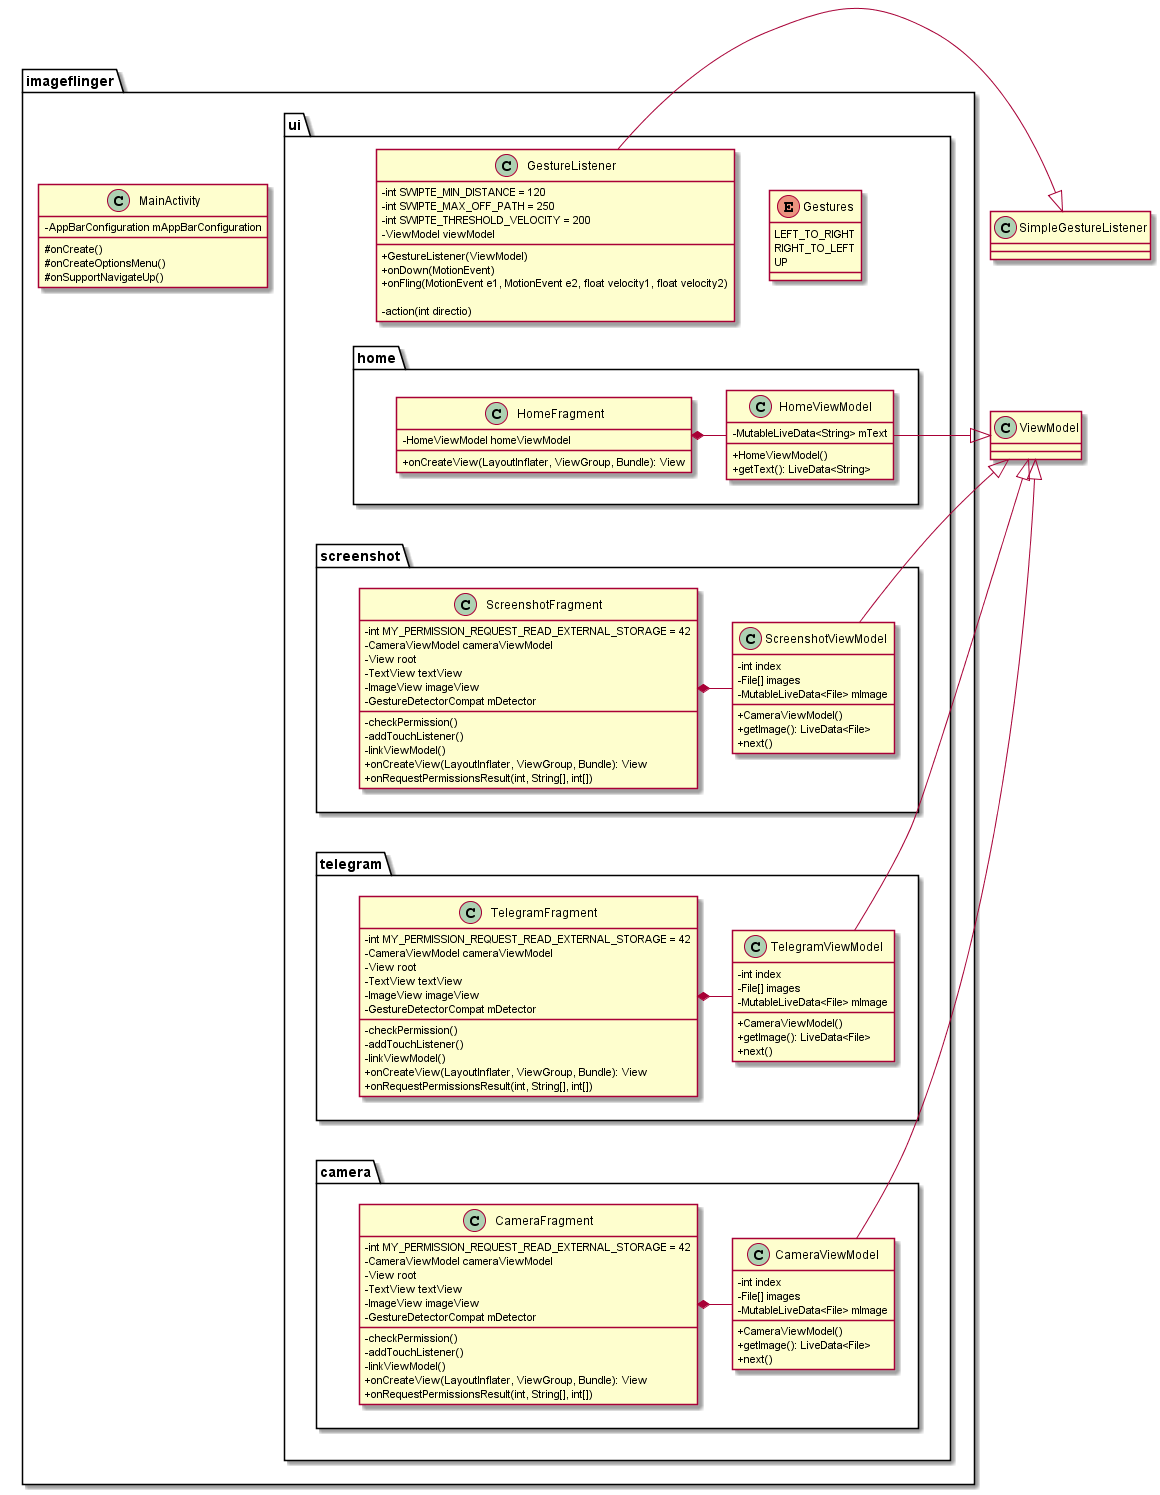
\includegraphics[width=1\linewidth]{figures/classdiagram.png}
    \caption{Architektur der Android-Applikation}
    \label{fig:Architektur}
\end{figure}

\section{Android-App}

\begin{figure}[H]
    \centering
    \begin{subfigure}[b]{0.3\linewidth}
      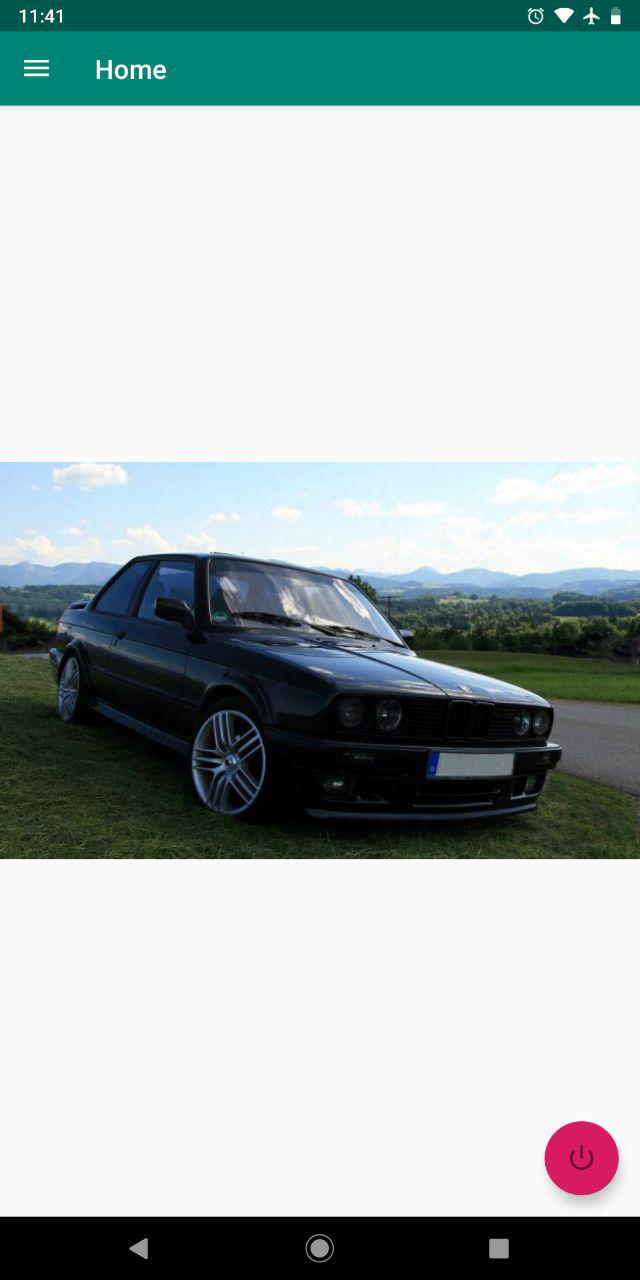
\includegraphics[width=1\linewidth]{figures/home.jpg}
      \caption{Startbildschirm}
    \end{subfigure}
    \begin{subfigure}[b]{0.3\linewidth}
      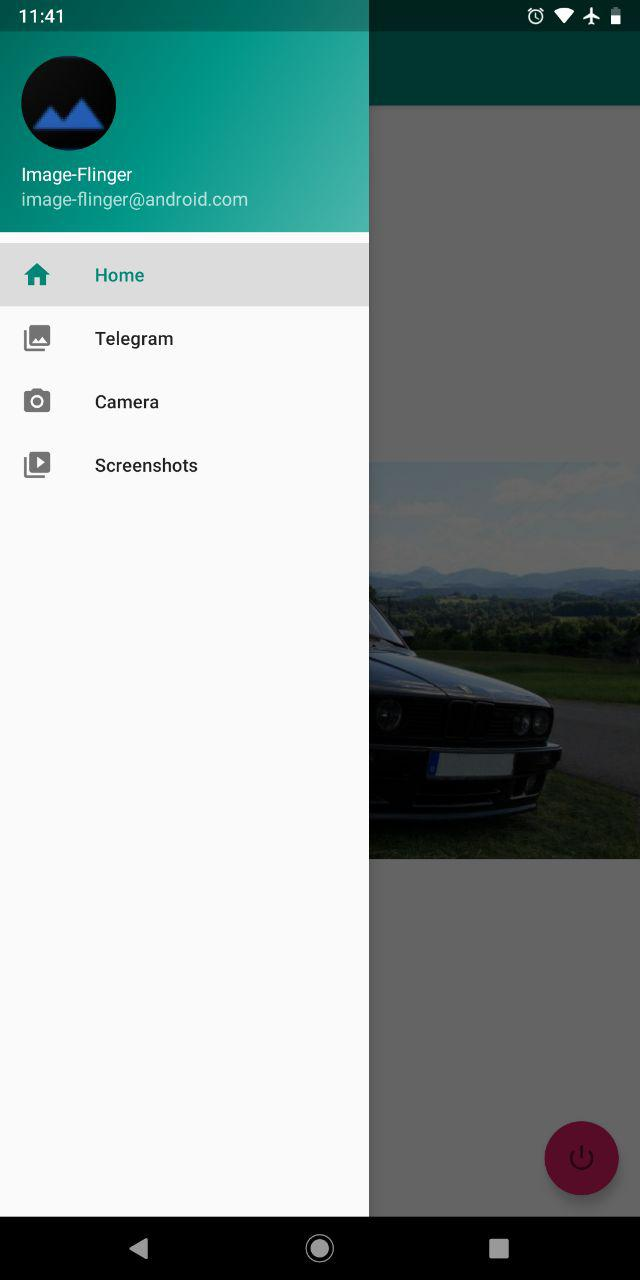
\includegraphics[width=1\linewidth]{figures/nav.jpg}
      \caption{Navigationsleiste}
    \end{subfigure}
    \caption{Startbildschirm und Navigationsleiste}
    \label{fig:start_nav}
\end{figure}


\begin{figure}[H]
  \begin{subfigure}[b]{0.3\linewidth}
    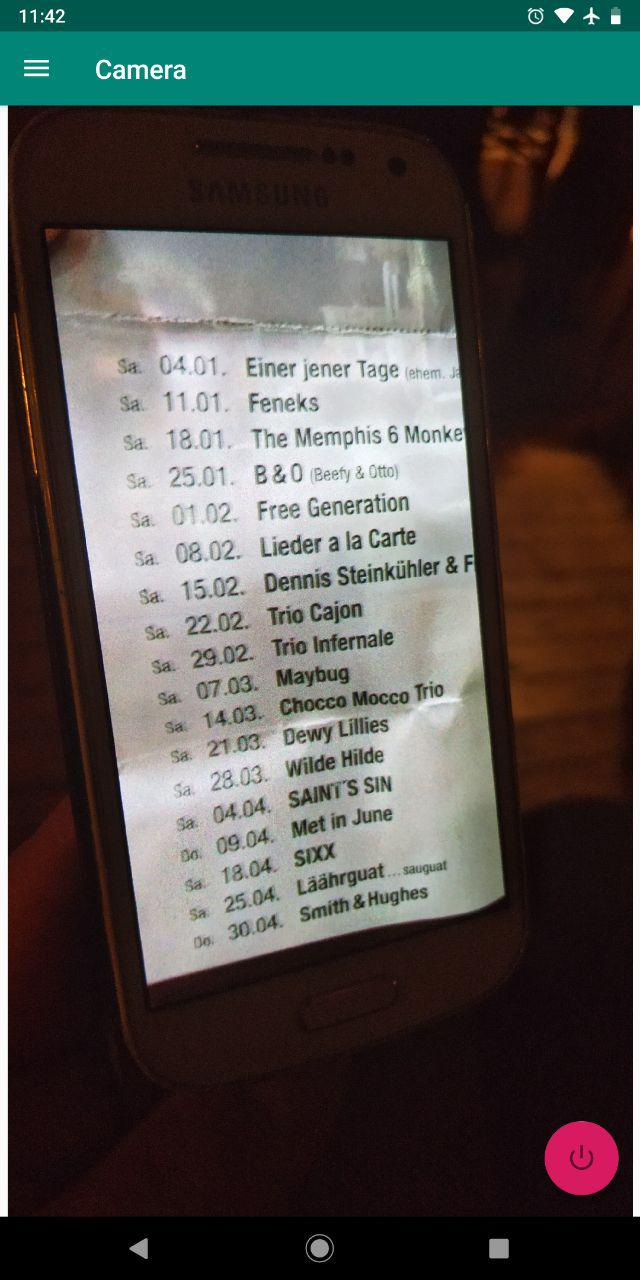
\includegraphics[width=1\linewidth]{figures/camera.jpg}
    \caption{Kamera}
  \end{subfigure}
  \begin{subfigure}[b]{0.3\linewidth}
    
\includegraphics[width=1\linewidth]{figures/telegram.jpg}
    \caption{Telegram}
  \end{subfigure}
  \begin{subfigure}[b]{0.3\linewidth}
    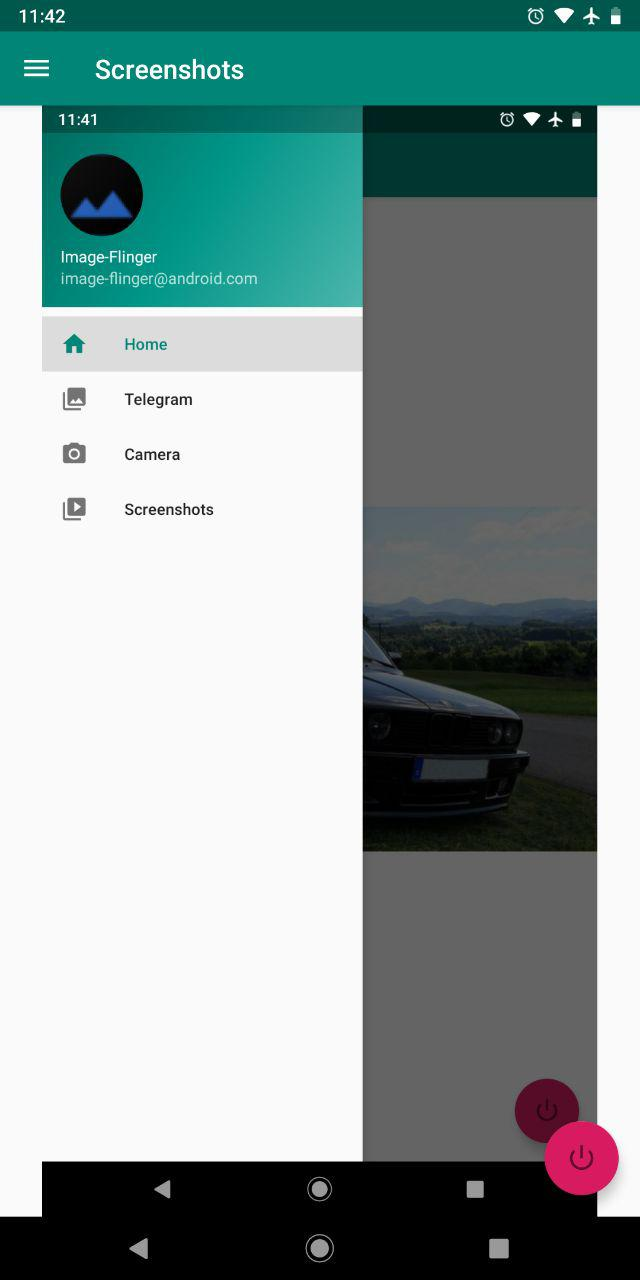
\includegraphics[width=1\linewidth]{figures/screenshots.jpg}
    \caption{Screenshots}
  \end{subfigure}
  \caption{Bilderverzeichnisse}
  \label{fig:folders}
\end{figure}

\newpage
% \section{Abbildungsverzeichnis}
\listoffigures
\newpage

% \section{Auflistungen}
% \lstlistoflistings

\end{document}

